\chapter{A cognitive approach to represent automotive scenes}%
\label{chap:a_cognitive_approach_to_represent_automotive_scenes}

We have seen in chapter ~\ref{chap:research_context}, especially in section ~\ref{subsec:knowledge_representation}, that, already today, there is a plethora of \acfp{ADAS} in intelligent vehicles. 
In future vehicles, the number of modules tackling different sub-tasks necessary to enable (semi-) autonomous driving and to interact with humans inside and outside the car will increase even more.
Given the complexity of the physical world and the recent success of \acp{DNN} in the diverse applications, a substantial amount of such modules could be data-driven with increasingly large neural networks under the surface.
In a worst case scenario, each of these systems will encapsulate its own representation of knowledge about the data it processes in complete separation from other, potentially related systems.
Typically, the representations used rely completely on numerical values and lack possibilities to be enriched or combined with symbol-like representations.
On the other hand, increasingly deep neural network architectures are not only hungry for data to generalize sufficiently enough from the examples they have been trained on, but also tend to require a substantial amount of computational resources.
Although this aspect is more severe for the training process, it becomes more important for mobile applications such as automated vehicles during the deployment phase.

In this thesis, we propose a novel representation for automotive scenes based on modern cognitive modeling techniques, namely the \ac{SPA}.
The \ac{SPA} is one particular example from a family of cognitive architectures commonly referred to as \acp{VSA} (see section ~\ref{subsec:vector_based_approaches} and chapter ~\ref{chap:introduction_to_vsas} for further details).
One of the key components of these cognitive architectures is to use high-dimensional vectors for representation.
This representational approach offers several desirable features.
High-dimensional vectors are one variant of distributed representations in the sense, that information is captured over all dimensions of the vector instead of one single number.
This aspect makes distributed representations more robust to noise in the sense, that a few noisy entries influence the overall information carried by the vector less compared to low-dimensional representations.
Furthermore, vector representations allow to encode both, symbol-like and numerical structures in a similar and unified way.
Additionally, the algebraic operations enable manipulation and combination of represented entities into structured representations.
One potential advantage of this approach is that the number of dimensions remains fixed independent of the number of entities combined through the architecture's algebraic operations.
Finally, vectors are a suitable representational substrate to be used in combination with neural networks.
On the one hand, vectors are a natural input to classic \acp{ANN}, but they also offer the possibility to be efficiently implement in \acp{SNN} using the principles of the \ac{NEF} (see \cite{Eliasmith2013}, but also section ~\ref{subsec:implementation_in_snns}).
Given an widespread implementation of the representations proposed here in combination with \acp{SNN} as algorithmic substrate within intelligent vehicles, the latter offers the potential to deploy such neural representations on dedicated neuromorphic hardware (cf.\ section ~\ref{sec:neuromorphic_HW}).
Although neuromorphic computing hardware as well as the corresponding neural algorithms are mainly used in academic research and often lack the technical maturity required by industrial applications, they show promise to be an energy-efficient option for future automated vehicles once reaching the required level of maturity.

\begin{figure}[t]
    \centering
    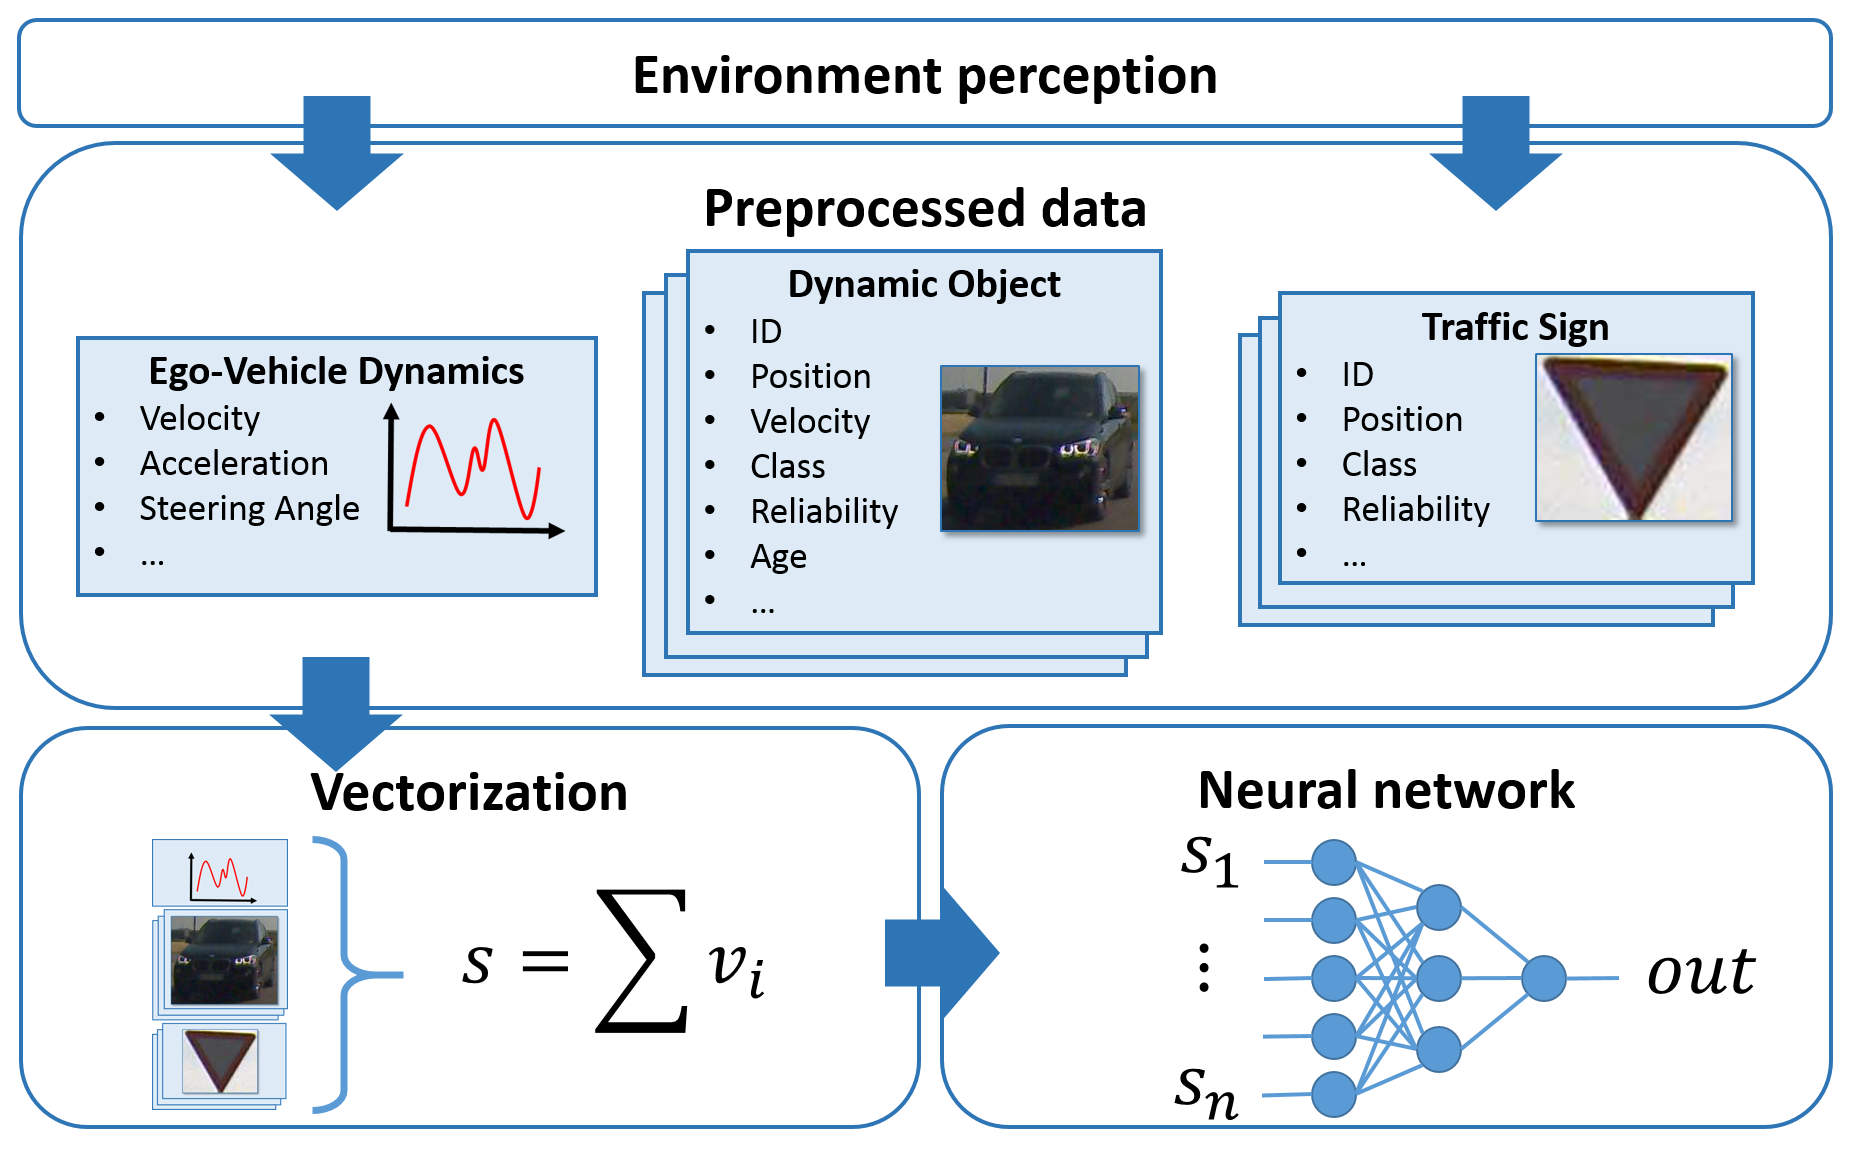
\includegraphics[width=0.8\linewidth]{imgs/system_overview_horizontal.eps}
    \caption{Visualization of the general flow of information of our proposed approach.}
    \label{fig:vectorization}
\end{figure}

In this chapter, we introduce our proposed approach to encapsulate high-level information about automotive scenes in high-dimensional, semantic vectors using the \ac{SPA} as representational substrate.
For this encoding phase, we follow the first two stages, namely \emph{preprocessing} and \emph{representation generation}, of the three-stages process established in \cite{Gallant2013} 
The third and final stage, \emph{output computation}, will be subject of subsequent chapters, where we investigate concrete applications and use cases.
The preprocessing stage is the step of creating a suitable vector vocabulary, whereas the representation generation stage is the process of building up structured representations from the atomic vectors within the vocabulary.
Furthermore, we analyze how different types of data could be encoded in such a representation, we show possible variations of how to encapsulate data in vectors and how they influence the final representation.
We also investigate potential limitations imposed bu such representations to provide insights into how many concepts can be efficiently encoded in our representations without loss of information.  


\section{Preprocessing stage - generating a vocabulary}%
\label{sec:preprocessing_stage_generating_a_vocabulary}

Fig. ~\ref{fig:vectorization} visualizes the general flow of information of our proposed system.
To represent high-level information about a scene in an abstract vector representation, we work with already processed data, which comes either from individual sensors, which perform their own low-level processing, or from a higher-level, central module already fusing information from several sensors.
We simply refer to this step as \emph{environment perception} in fig. ~\ref{fig:vectorization}, whereas its output is referred to as \emph{preprocessed data}.
This data is typically available as lists of objects present in the current scene and is translated into a semantic vector representation by first assigning atomic vectors to entities of interest and then building up more complex, structured representations by using the \ac{SPA}'s algebraic operations.
In this section, we will investigate the first step of assigning atomic vectors to entities of interest, i.e., creating a suitable vector vocabulary.
We have already seen in section ~\ref{subsec:vocabs}, that such vocabularies can be created in several different ways, which we will investigate with the specific focus of encoding automotive scenes.

\subsection{What types of data to encode?}%
\label{subsec:what_types_of_data_to_encode_}

The data to be encoded in a semantic vector substrate depends not only on the information available from the current sensor-setup, but also on the task at hand.
For instance, if we want to classify the current driving context (like in chapter ~\ref{chap:driving_context_classification}), the relevant information might be different to the task of predicting a vehicle's trajectory (like in chapter ~\ref{chap:behav_pred}).
Here, we give an overview of what information in general is available in an intelligent vehicle and how to encode it in a semantic vector substrate.
We distinguish between symbol-like information such as the type of a dynamic object or numerical information such as the current acceleration of the ego-vehicle.
In this section, we focus mainly on the symbol-like information, which is suitable to be represented using a single atomic vector or an algebraic combination of several atomic vectors.
In section ~\ref{subsec:different_vector_representations_for_numerical_values}, we will focus on numerical information and different options of encoding them in vectors,
Here, we will closely follow the structure of section ~\ref{sec:cognitive_modelling_with_vsa} and present different possibilities to generate a vocabulary of atomic vectors to built structured representations upon.

If the vectors in the vocabulary are not chosen at random, the general goal when creating the vocabulary is to generate atomic vectors that carry inherent structure or meaning.
This meaning is typically reflected by similar concepts being mapped to similar vectors.
However, there are several possible notions of similarity that can be encoded in the vocabulary, which we will specify in this section.

\subsubsection{Visual similarity}%
\label{ssubsec:visual_similarity}

A first simple and comprehensible notion of similarity is visual similarity between two entities: "do they look similar". 
Encoding this notion in vectors, we would expect the vector representations to represent this type of similarity within the relation between the vectors, meaning that vectors representing visually similar entities will have large cosine similarity.
In conjunction with other information, this type of similarity could be useful to detect a wrong classification, in case it has high similarity to another one that makes more sense in the situation or context at hand.
An example would the German traffic signs indicating a speed limit of \SI[per-mode=symbol]{30}{\kilo\meter\per\hour} and \SI[per-mode=symbol]{80}{\kilo\meter\per\hour}, which are both circular with a red frame and a similar looking black number on white background in the middle.
However, encountering a speed limit sign of \SI[per-mode=symbol]{30}{\kilo\meter\per\hour} in an urban situation is more plausible than a sign indicating a speed limit of \SI[per-mode=symbol]{80}{\kilo\meter\per\hour}.

\subsubsection{Similarity of motion}%
\label{ssubsec:similarity_of_motion}

Another notion of similarity, that is a candidate to be encoded in a vector vocabulary is the similarity of motion properties.
For instance, bicycles and motorcycles have more similar motion properties (dynamics of vehicles with two wheels) than for example a pedestrian and a truck.
Apart from motion properties such as dynamics of the movement, the number of wheels or the mean expected velocity the direction of movement of traffic participants can be a notion of similarity to be encoded in the vocabulary.
For instance, traffic participants such as bicycles or cars moving towards us might be encoded more similarly to each other than to parked cars or those moving away.
Furthermore, some entities are more likely to change their motion or direction: while traffic lights frequently alternate and parked cars might start moving, trees, buildings and traffic signs are expected to remain static. 
The notion of similarity of motion can be useful in various ways.
In a first step, knowing the motion of other traffic participants could help in classifying the situation: on a multi-lane highway we would expect cars around us to move in the same direction, whereas in an urban driving situation the motion of other traffic participants is more diverse. 
Additionally, this notion of similarity could potentially help in focusing the system's attention or more precisely, use computing power more efficiently on entities that are more relevant to decision making.
For example, a change of the 'motion status' (e.g.\ when a bus stops) might need particular attention.

\subsubsection{Semantic similarity}%
\label{ssubsec:semantic_similarity}

While visual similarity already captures a significant part of perceivable information about entities in automotive context, there is further information that could be encoded in the vector vocabulary that is different, and maybe even, contrary to visual similarity. 
Considering automotive situations, we as humans do not only assess them based on visual appearance but also by incorporating underlying and, most likely, previously acquired knowledge about the objects in the scene.
This underlying information can be considered the semantic aspect.
Revisiting the aforementioned example, the speed limit sign for \SI[per-mode=symbol]{30}{\kilo\meter\per\hour} is \emph{viusally} more similar to \SI[per-mode=symbol]{80}{\kilo\meter\per\hour} than to \SI[per-mode=symbol]{20}{\kilo\meter\per\hour}.
However, in the context (or semantics) of an automotive situation such as driving in an urban environment, speed limit signs for \num{20} and \SI[per-mode=symbol]{30}{\kilo\meter\per\hour} should be contextually or semantically more similar than signs for \num{30} and \SI[per-mode=symbol]{80}{\kilo\meter\per\hour}, as they are more likely to appear in similar contexts and both describe the traffic rule restricting driving to slow velocities.

Semantic similarity is not quite as intuitive as visual similarity. 
In general, we want to encode objects and concepts sharing similarity in \emph{meaning} in vectors with a high cosine similarity.
However, it is not intuitively clear what similar meaning actually refers to and how to properly define semantic similarity in an automotive context.
In the field of generating word embeddings for natural language processing, the typical assumption is that words that share similarity in meaning appear in close proximity with high probability within text corpora.
This assumption could be transferred to automotive context as well, for instance thinking of traffic signs indicating speed limits appearing in similar contexts or driving situations such as urban driving compared to higher speed limit signs.
However, on the one hand it is not clear how to transfer this approach to other object classes such as traffic participants whose appearance probability is less context dependent than for traffic signs. 
On the other hand the process of automatically training a system to learn this form of embedding is not clear as it would probably demand for another learning model to extract contextual information from the rich features of driving contexts.
Therefore, will now focus on the potential meaning of objects appearing in an automotive environment and how their semantic meaning could be embedded into a vector representation while leaving aside intangible concepts representing vehicle dynamics such as "velocity" or "acceleration".

\paragraph{Traffic signs}%
\label{par:traffic_signs}

Any traffic sign carries an explicit meaning defined in traffic law and anyone with a driver's license should know its meaning and be able to immediately explain it.
The meaning of a traffic sign is an instruction for the driver's behavior to, for instance, not surpass a certain velocity or to give way to other traffic participants. 
There are sub-groups of signs with similar meanings, such as signs indicating speed limits, prescribed direction or warnings for potentially dangerous road conditions or to pay increased attention.
Encoding the semantic structure of traffic signs in a vector vocabulary, we expect not only all traffic signs will be similar but also that all signs within a certain sub-group end up being more similar to one another compared to signs from other subgroups. 
For instance, signs indicating speed limits should be similar to one another, ideally with signs indicating lower velocities such as \SI[per-mode=symbol]{20}{\kilo\meter\per\hour} and \SI[per-mode=symbol]{30}{\kilo\meter\per\hour} should be more similar than \SI[per-mode=symbol]{30}{\kilo\meter\per\hour} and \SI[per-mode=symbol]{130}{\kilo\meter\per\hour}. 
Beside their explicit meaning, the number of traffic signs is finite and limited to a small number compared to the number of words in a typical human-level language vocabulary.
Therefore it is possible to manually engineer their semantic similarity, which makes it easier to impose our human understanding onto the structure, although the resulting vocabulary will most likely differ from the structure an unsupervised learning model would pick up from the data. 

\paragraph{Traffic participants}%
\label{par:traffic_participants}

While the meaning of traffic signs is clear and explicit, it is far more difficult to derive a meaning of a traffic participant such as a car or a pedestrian or a measure of similarity between them.
It is unclear if a truck is semantically more similar to a motorcycle or to a car without considering any contextual information while ignoring similarity of motion properties, which have already been discussed in section ~\ref{ssubsec:similarity_of_motion}.
However, if we do consider contextual information, we as humans decide intuitively if a truck and a motorcycle are more similar when compared to a pedestrian by e.g., considering their velocity of motion.
We also know from experience that the meaning of a car approaching from the right potentially means that it has the right of way when we encounter a situation at a crossroads without traffic signs indicating other right of way rules. 
Hence, the situational context has a significant impact on comprehending the "meaning" of traffic participants, which in most cases directly results in appropriate driving actions to take such as decelerating or changing the lane.
However, such a situational understanding is impossible to derive without additional information such as position, velocity or direction of each traffic participant.
Consequently, it is impossible to encapsulate such semantic or contextual similarity in a vector vocabulary directly but rather encode another notion of similarity for atomic vectors of traffic participants and built situational similarity through structured representations using the \ac{VSA}'s algebraic operations.

\subsubsection{Summary on similarity}%
\label{ssubsec:summary_similarity}

All of the aforementioned notions cover a certain aspect of similarity.
Ideally, it is desirable for a vector vocabulary to encapsulate more than one notion of similarity comparable to a human understanding all these different aspects of similarity.
However, it is not clear if it is helpful or even possible, to encapsulate several notions of similarity into one coherent vector vocabulary or if it is more suitable to have separate vocabularies for each similarity of interest and combine them in structured representations using the \ac{VSA}'s algebraic operations as mentioned e.g., in \cite{Crawford2016}.
For the remainder of this section, we give an overview over different options of how to generate vector vocabularies encoding their own notion of similarity.

\subsection{Random and manually engineered vocabularies}%
\label{subsec:basic_random_vocabularies}

The simplest possible option to generate a vocabulary of atomic vectors is to sample them randomly, in case of continuous \acp{VSA} such as the \ac{SPA}, from the $D$-dimensional unit sphere \cite{Voelker2017}.
Naturally, randomly chosen atomic vectors do not carry semantic meaning or any intended notion of similarity.
However, given a sufficiently large dimension $D$ of the chosen \ac{VSA} and its theoretical properties (see chapter ~\ref{chap:introduction_to_vsas}), we can assume that randomly chosen vectors will be dissimilar enough to avoid accidentally mistaking them for one another.
Another advantage of this simple approach is that is comparatively easy to create a vocabulary avoiding any complex learning system to embed the concepts of interest in semantic vectors.
On the other hand, if specific applications demand for the vectors to actually carry semantic information meaning that similar concepts need to be mapped to similar vectors for the application to succeed, this simple approach can be extended by manually engineering a vocabulary reflecting the desired similarity structure.
This is typically achieved by randomly choosing a set of auxiliary vectors and building atomic vectors with the desired similarity from them through the \ac{VSA}'s algebraic operations (cf.\ section ~\ref{subsec:vocabs}).
However, this approach is only feasible and appropriate for rather small sized vocabularies as manually designing semantic vectors with certain similarity properties becomes intractable quickly with an increasing number of concepts to be embedded.
Furthermore, manually designing vocabularies involves design choices by human engineers, which is sensitive to potentially undesired biases in the similarity structure of the vectors.
For instance, the example vocabulary created in section ~\ref{subsec:vocabs} solely focused on the motion characteristics and typical actuators of different traffic participants.
However as mentioned before, there are many other possible similarity structures such as visual (or auditory), motion or semantic similarity, to be considered when designing the vocabulary.

\subsection{Visual vocabularies}%
\label{subsec:visual_vocabularies}

\subsection{Pre-learned semantic vocabularies}%
\label{subsec:pre_learned_semantic_vocabularies}

\subsection{Visual-semantic vocabularies}%
\label{subsec:visual_semantic_vocabularies}

results from Roberts thesis

\section{Representation generation stage}%
\label{sec:representation_generation_stage}


\subsection{Different vector representations for numerical values}%
\label{subsec:different_vector_representations_for_numerical_values}


In this section, we investigate different approaches to map numerical information to semantic vectors.
Therefore, we will focus on
problem of how to encode numerical information (vector length vs trigonomical vs. unitary vector powers) for values of position, velocity etc.
\subsubsection{Scalar multiplication encoding}
\subsubsection{Sine and Cosine encoding with different frequencies and offsets}
For vectorization of two-dimensional values, we use an encoding with sine and cosine functions with different spatial frequencies and offsets.
Therefore, we define the following helper functions
\[ \abb{f_{\left(m,i\right)}}{\mathbb{R}^2}{\mathbb{R}^4}{\left(x,y\right)}{\left(\cos\frac{m\cdot \pi + x}{i + 1}, \sin\frac{m\cdot \pi + x}{i + 1}, \cos\frac{m\cdot \pi + y}{i + 1}, \sin\frac{m\cdot \pi + y}{i + 1}\right)},
\]
\[
\abb{\psi_i}{\mathbb{R}^2}{\mathbb{R}^4}{\left(x,y\right)}{\left(f_{\left(0,i\right)}\left(x,y\right), f_{\left(\frac{1}{2},i\right)}\left(x,y\right), f_{\left(1,i\right)}\left(x,y\right), f_{\left(\frac{3}{2},i\right)}\left(x,y\right)\right)}
\]
and obtain the final vector representation of acceleration in $x$/$y$-direction via the function
\[
\abb{\lambda}{\mathbb{R}^2}{\mathbb{R}^D}{\left(x,y\right)}{\frac{1}{\sqrt{\frac{D}{2}}}\left(\psi_0\left(x,y\right), \cdots, \psi_{\frac{D}{16}-1}\left(x,y\right)\right).}
\]
This encoding $\lambda\left(a_x, a_y\right)$ leads to normalized, nonzero, similar vectors with information distributed over all elements (in contrast to a simple encoding like $\left(a_x, a_y, 0 \cdots, 0\right)$).
\subsubsection{Convolutive power encoding}

\subsection{Structured representations}%
\label{subsec:structured_representations}

\section{Capacity analysis - limitations to vector representations}%
\label{sec:capacity_analysis_limitations_to_vector_representations}

\subsection{Limiting factors to structured representations}%
\label{subsec:limiting_factors_to_structured_representations}


\begin{figure}[t]
	\centering
	\includegraphics[width=0.95\textwidth]{imgs/spa_superposition_capacity_1.png}
	\caption{Superposition capacity.}
	\label{fig:spa_superposition_capacity}
\end{figure}

\section{Summary}%
\label{sec:vector_representations_automotive_summary}
\todo[inline]{somewhere (maybe in one of the subsequent chapters) where it is fitting the option to adjust the vector embedding based on the performance on a certain task to potentially improve the model's task performance by a better vector embedding (something more of future work thing, not intended to be investigated in this thesis, but still worth mentioning)}


